\chapter{Technologie i pojęcia wykorzystane w projekcie  }
\label{cha:Technologie}
W poniższym rozdziale przedstawiono zagadnienia 

\section{Obraz całkowy}
\label{sec:IntegralImage}
Obraz całkowy (z ang. \textit{Integral Image} \cite{ViolaJonesIntegralImage}) to struktura danych wykorzystywana w celu efektywnej i szybkiej generacji sum pikseli dla podanego regionu obrazu. Dowolny piksel \textit{(x, y)} obrazu \textit{I} może zostać przedstawiony jako suma wszystkich pikseli na lewo oraz powyżej \textit{(x, y)}:
\begin{equation}
\textit{Obraz całkowy}(x^{'},y^{'}) = \sum_{x<x^{'},y<y^{'}}^{}I(x,y).
\end{equation}

Użycie takiej reprezentacji umożliwia uzyskanie sumy pikseli dowolnego obszaru obrazu w stałym czasie, bez względu na jego rozmiar. Dodatkowo wyliczenie obrazu całkowego następuje w pojedynczym przejściu po pikselach. Wynika to z faktu, że kolejne elementy struktury są tworzone na podstawie już istniejących. Przykład wykorzystania obrazu całkowego  przedstawiono na rysunku \ref{im: Integral Image} 

\begin{figure}[h]
	%\centering
	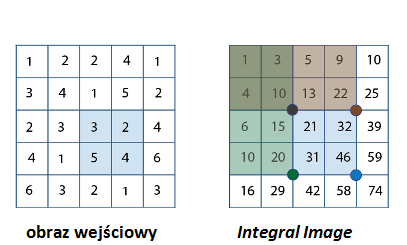
\includegraphics[width=12cm]{integral_image}
	\centering
	\caption{Zasada wyliczania obrazu całkowego}
	\label{im: Integral Image}
\end{figure}    

Wyliczenie sumy wyróżnionego regionu na obrazie wejściowym można zastąpić operacjami na obrazie całkowym. Sumę obszaru można uzyskać korzystając z czterech wartości powyżej oraz na lewo od zaznaczonych kropek: \textit{46 - 22 - 20 + 10 = 14}. Jak nietrudno obliczyć, wynik ten jest równy sumie zaznaczonych elementów obrazu wejściowego.

\section{Ciągła przestrzeń skali dla obrazu}
\label{sec:StateSpace}
W cyfrowym przetwarzaniu obrazów model ciągłej przestrzeni skali może zostać użyty do reprezentacji obrazu jako rodziny stopniowo rozmywających się obrazów. Wykorzystanie ciągłej przestrzeni skali umożliwia znalezienie punktów na obrazie, które są niewrażliwe na zmiany skali (z ang. \textit{scale invariant}). 

To zagadnienie jest bardzo ogólne i istnieje wiele reprezentacji przestrzeni skali. Typowym podejściem do zdefiniowania szczególnej reprezentacji przestrzeni skali jest zdefiniowanie zbioru aksjomatów opisujących podstawowe własności szukanej przestrzeni. Najbardziej powszechnym zbiorem aksjomatów jest zbiór definiujący liniową przestrzeń skali powiązaną z funkcją Gaussa. 

\begin{figure}[h]
	%\centering
	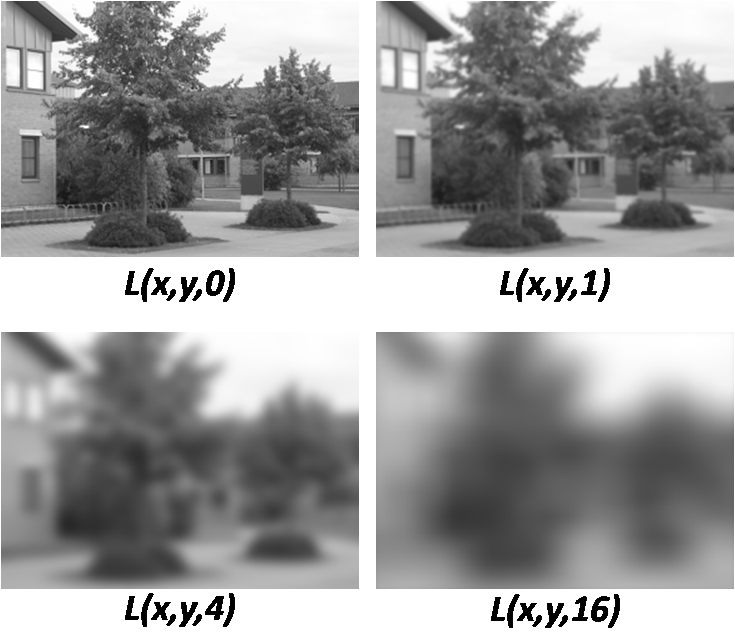
\includegraphics[width=10cm]{ScaleSpaceRepresentation}
	\centering
	\caption{Reprezentacja przestrzeni skali dla różnych wartości $\sigma$}
	\label{im: Scale Space Representation}
\end{figure} 

Problem sprowadza się do znalezienia takiego zbioru operatorów $\tau_s$, który operaując na obrazie oryginalnym zdefiniuje zbiór obrazów rozmytych:  

Gaussowska przestrzeń skali (dla obrazu dwuwymiarowego) zdefiniowana jest jako splot obrazu \textit{I(x,y)} z dwuwymiarową funkcją Gaussa \textit{g(x,y,$\sigma$)}:
\begin{equation}
L(x,y,\sigma) = g(x,y,\sigma)*I(x,y)
\end{equation}
gdzie:
\begin{equation}
g(x,y,\sigma) = \frac{1}{2\pi\sigma}e^{-(x^2+y^2)/2\sigma}
\end{equation}

%Podany wzór spełniony jest dla \textit{$\sigma$$\geq$0}
Dla $\sigma = 0$ filtr Gaussa staje się funkcją impulsową, zatem \textit{L(x,y,0) = f(x,y)}. Wraz ze zwiększaniem parametru $\sigma$ przestrzeń skali \textit{L} staje się coraz bardziej rozmyta, czyli coraz mniej szczegółów przestaje być widoczne. Na rysunku \ref{im: Scale Space Representation} przedstawiono przykład tworzenia przestrzennej reprezentacji skali.

\section{Windows Presentation Foundation (WPF)}
Windows Presentation Foundation jest silnikiem graficznym dostarczanym przez firmę Microsoft. Jego premiera nastąpiła w 2006 roku, gdy stał się częścią platformy programistycznej .NET w wersji 3.0.  Jest wykorzystywany głównie do budowania aplikacji okienkowych nowej generacji dla systemu opracyjnego Windows. WPF zbudowany został całkowicie niezależnie do dotychczasowego silnika renderujacego GDI. Dostarcza model programistyczny umożliwiajacy budowanie aplikacji oraz pozwalający na bezwzględną separację logiki biznesowej od interfejsu użytkownika. 

\begin{figure}[h]
	%\centering
	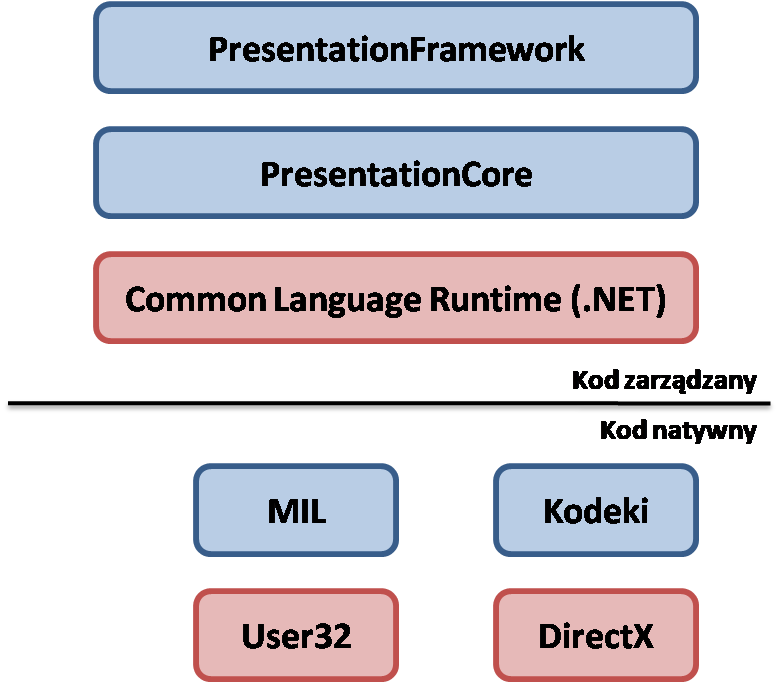
\includegraphics[width=10cm]{WpfArchitecture}
	\centering
	\caption{Architektura WPF. Czerwone elementy to komponenty bibliotek Windows. SKładowe WPF oznaczono kolorem niebieskim.}
	\label{im: WpfArchitecture}
\end{figure} 

Architektura silnika WPF została oparta zarówno o kod zarządzany, jak i o kod natywny.  Większość elementów składowych znajduje się w kodzie zarządzanym, tak jak publiczne API dostępne dla deweloperów. Na rysunku \ref{im: WpfArchitecture} przedstawiono architekturę silnika, w skład którego wchodzą:

\begin{itemize}
	\item PresentationFramework – biblioteka implementująca elementy do prezentacji dla końcowego uzytkownika tj. rozkład kontrolek, wyświetlanie animacji, skalowanie aplikacji. 
	
	\item PresentationCore – podstawowa biblioteka w technologii WPF. Dostarcza wraper dla MIL z poziomu kodu zarządzanego oraz impementuje bazowe  usługi dla każdej aplikacji WPF. W skład tych usług wchodzi przede wszystkim system zarządzania wiadomościami , którego implementację stanowi obiekt typu Dispacher.  
	
	\item Media Integration Layer, MIL – komponent działający w kodzie niezarządzanym w celu zapewnienia wydajnej współpracy  z DirectX.   Zawiera silnik kompozycji, który odpowiada za  podstawową obsługę renderowania powierzchni 2D oraz 3D.
	
	\item Kodeki – zbiór programów odpowiedzialnych do przekształcania strumienia danych do postaci multimedialnej.
	
	\item DirectX – kolekcja zawierająca interfejsy programistyczne aplikacji (z ang. application programming interfaces, APIs). Zestaw ten  wspomaga generację grafiki, dźwięku oraz innych elementów związanych z aplikacjami multimedialnymi
	
	\item User32 – komponent Microsoft Windows dostarczający bazowe funkcjonalności do tworzenia prostych interfejsów użytkownika.  Aplikacje WPF zawierają obiekt typu Dispacher, który używa systemu zarządzania wiadomościami dostępnymi w User32.
	
	\item Common Language Runtime, CLR – wspólne środowisko uruchomieniowe. Podstawowy komponent .NET. Pelni wiele kluczowych roli tj. uruchomienie aplikacji, zarządzanie pamięcią. Dodatkowo zajmuje się również konwersja języka IL do kodu maszynowego. Elementem bazowym środowiska CLR jest standardowy zestaw typów danych, który jest wykorzystywany przez wszyskie języki programowania oparte o CLR. 
	
\end{itemize}

Silnik WPF udostępnia system własności dla obiektów, które dziedziczą z DependencyObject. Obiekt ten monitoruje  wszytkie zależności pomiędzy własnościami i jest w stanie wykonywać odpowiednie akcje bazujac na ich zmianach. Własności implementują mechanizm informujący o zmianach (z ang. Change notifications), który wywołuje wbudowane zachowania (z ang. Behaviors) w przypadku wykrycia jakiejkolwiek zmiany. Dodatkowo isniej możliwość definiowania własnych zachowań w celu propagowania informacji o zmianie własności do innych elementów . System zarządzania rozkładem elementów w obrzarze interfejsu użytkownika wykorzystuje powyższy zbior zachowań do przeliczania nowego rozkładu w przypadku zmiany własności. Dzięki temu architektura systemu WPF spełnia deklaratywny paradygmat programowania, w którym praktycznie wszystko, począwszy od ustawania wielkości kontrolek do tworzenia animacji może zostać osiągnięte poprzez zmianę własności. Takie zachowanie umożliwia tworzenie aplikacji WPF w XAML (z ang. Extensible Application Markup Language) – deklaratywnym języku znaczników, gdzie przy pomocy atrybutów oraz słów kluczowych tworzone jest bezpośrednie połączenie z własnościami oraz klasami technologii WPF. 

Każdy element interfejsu aplikacji WPF dziedziczy z abstrakcyjnej klasy Visual. Obiekty tej klasy dostarczają interfejs do drzewa kompozycji zarządzanego przez MIL. Każdy element WPF tworzy oraz dodaje przynajmniej jeden węzeł kompozycji do drzewa. Węzły te zawierają przede wszystkim instrukcje renderowania takie jak przycinanie elementu bądź transformacja wizualna. Zatem cała aplikacja może być traktowana jako kolekcja węzłów kompozycji, które są przechowywane w buforze pamięci. Okresowo MIL przechodzi po strukturze drzewa i wykonuje instrukcje renderowania dla każdego węzła. Powoduje to tworzenie kompozytu na powierzchni DirectX, która następnie jest wyświetlana na ekranie.  MIL wykorzystuje algorytm malarza, w którym wyświetlanie elementów na monitorze rozpoczyna się od tych najbardziej odległych (tło). Takie zachowanie umożliwia renderowanie złożonych efektów takich jak rozmycie czy transparentność. Dodatkowo proces rysowania jest sprzętowo wspomagany przy pomocy GPU. 

Każda z aplikacji WPF staruje z dwoma wątkami: pierwszy służy do obsługi interfejsu użytkownika, a drugi, działający w tle, obsługuje renderowanie oraz przerysowywanie – jego działanie jest automatyczne, więc nie wymaga żadnej interwencji dewelopera. Wątek powiązany z UI przechowuje obiekt Dispacher’a (poprzez instancję klasy DispacherObject), który zajmuje się kolejkowaniem operacji koniecznych do wykonania na interfejsie użytkownika.

Etap tworzenia układu interfejsu użytkownika podzielony jest na dwie fazy: Mierzenie (z ang. Measure) oraz Porządkowanie (z ang. Arrange). Faza mierzenia rekursywnie wywołuje wszystkie elementy określa rozmiar, z jakim one będą wyświetlane. Porządkowanie to faza, podczas której następuje rekursywne układanie wszystkich elementów w stosunku do ich rodziców w drzewie kompozycji. 


\section{Algorytm SURF}
Algorytm SURF (skrót od ang. \textit{Speeded Up Robust Features}) został opatentowany przez grupę naukowców w 2007 roku [BIBLIOGRAFIA]. Należy do rodziny algorytmów bazujących na punktach kluczowych i służy do porównywania dwóch obrazów operując w odcieniach szarości. W celu znalezienia cech obrazu niezależnych od zmiany skali wykorzystuje opisaną w podrozdziale \ref{sec:StateSpace} technikę utworzenia ciągłej przestrzeni skali opartej na rozkładzie Gaussa. Dodatkowo algorytm ten dzieli przestzeń skali na poziomy oraz oktawy. Oktawa odpowiada zbiorowi splotów, w którym wartość parametru $\sigma$ zostaje podwojona. Każda oktawa podzielona jest na jednakowo odległe (ze względu na parametr $\sigma$) poziomy. Przykład przedstawiono na rysunku \ref{im: OctavesAndLevels}.
\begin{figure}[h]
	%\centering
	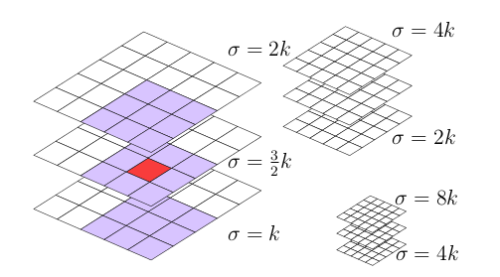
\includegraphics[width=10cm]{OctavesAndLevels}
	\centering
	\caption{Trzy oktawy z trzema poziomami. Szukanie cech obrazu obejmuje sąsiedztwo badanego punktu.}
	\label{im: OctavesAndLevels}
\end{figure}

Działanie algorytmu można podzielić na 3 etapy:

\begin{itemize}
	\item Detekcja (z ang. \textit{Detection}) – faza automatycznej identyfikcji punktów kluczowych (z ang. \textit{interest points}). Te same punkty powinny zostać wykryte niezależnie od zmian w położeniu, naświetleniu oraz orientacji obrazu, również w pewnym stopniu od zmiany skali oraz punktu widzenia. 
	\item Opis (z ang. \textit{Description}) – każdy punkt kluczowy powinien zostać opisany w unikatowy sposób., aby był niezależny od rotacji oraz przeskalowaniu obrazu.
	\item Zestawienie (z ang. \textit{Matching}) – faza, podczas której określa się (na podstawie podanych punktów kluczowych) jakie obiekty znajdują się na obrazie. 
\end{itemize}

W dalszej części rozdziału przedstawiono bardziej dokładną analizę dwóch pierwszych etapów.

\subsection{Detekcja}
Algorytm SURF do wykrycia punktów kluczowych wykorzystuje aproksymację wyznacznika Hesjanu. Najważniejszy element detekcji to proces polegający na ograniczaniu lokalnych wartości niemaksymalnych (z ang. \textit{non-maximal suppression}) dla wyznaczników macierzy Hessego przy różnych wartościach parametru $\sigma$. W celu redukcji czasu obliczeń korzysta z obrazu całkowego opisanego w podrozdziale \ref{sec:IntegralImage}.
Mając do dyspozycji punkt \textit{\textbf{x}=(x,y)} z obrazu całkowego, macierz Hessego \textit{H(\textbf{x},$\sigma$)} dla skali $\sigma$ jest zdefiniowana następująco:
\begin{equation}\textsl{}
H(\textbf{x},\sigma) = 
\begin{bmatrix}
L_{xx}(\textbf{x},\sigma) & L_{xy}(\textbf{x},\sigma) \\ L_{xy}(\textbf{x},\sigma) & L_{yy}(\textbf{x},\sigma)
\end{bmatrix}
\end{equation}

gdzie 
\begin{equation}\textsl{}
L_{xx}(\textbf{x},\sigma) = I(\textbf{x})*\frac{\delta^2}{\delta x^2}g(\sigma)
\end{equation}
\begin{equation}\textsl{}
L_{xy}(\textbf{x},\sigma) = I(\textbf{x})*\frac{\delta^2}{\delta xy}g(\sigma)
\end{equation}

Udowodniono, że przestrzeń skali oparta o funkcję Gaussa jest rozwiązaniem optymalnym {BIBLIOGRAFIA}, jednakże w zastosowaniach praktycznych wyliczanie splotu jest niezwykle kosztowne obliczeniowo. W celu przyspieszenia obliczeń dokonano aproksymacji drugich pochodnych cząstkowych filtrami przedstawionymi na rysunku \ref{im: GaussianApproximation}. Dodatkowo wykorzystanie obrazu całkowego powoduje, że czas wyliczania splotów nie zależy od wielkości filtra. 
\begin{figure}[h]
	%\centering
	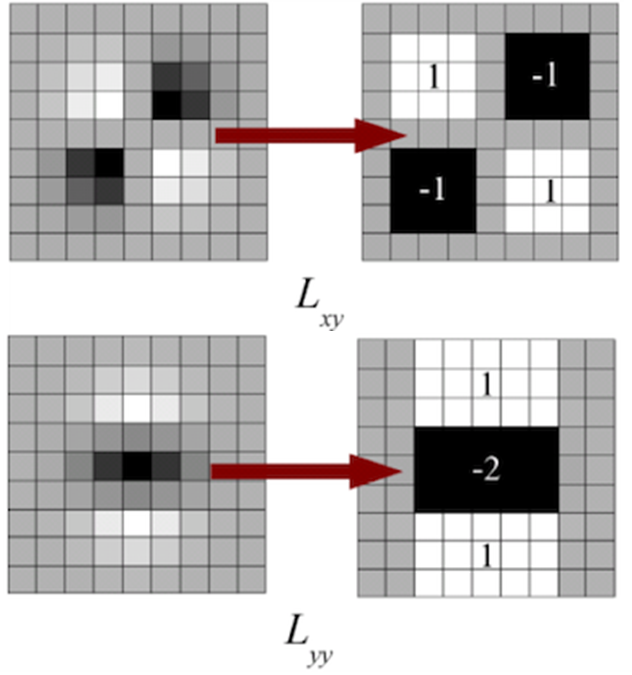
\includegraphics[width=8cm]{SurfLxyLyy}
	\centering
	\caption{Dwa rysunki po lewej to sploty \textit{$L_{xy}$} oraz \textit{$L_{yy}$} poddane dyskretyzacji oraz przycięciu. Po prawej stronie przedstawiono aproksymacje wyżej wymienionych splotów (odpowiednio \textit{$D_{xy}$} oraz \textit{$D_{yy}$}). Szare regiony są równe zero [BIBLIOGRAFIA]}
	\label{im: GaussianApproximation}
\end{figure}
Przedstawione aproksymacje odpowiadają splotom, dla których parametr $\sigma$ jest równy 1.2. Jest to najmniejsza wartość skali, dla której algorytm SURF może dawać zadowalające rezultaty.

Biorąc pod uwagę powyższe założenia, wyznacznik aproksymowanej macierzy Hessego wynosi:
\begin{equation}\textsl{}
det(H_{aproks}) = D_{xx}D_{yy} - (wD_{xy})^2.
\end{equation}
Aby uczynić aproksymację Hesjanu bardziej dokładną wprowadzono parametr \textit{w}. Teoretycznie jest on zależny od skali, jednakże badania wykazały [BIBLIOGRAFIA], że można uczynić go stałą równą \textit{0.9}.  

Najważniejszy element detekcji to proces polegający na ograniczaniu lokalnych wartości niemaksymalnych (z ang. \textit{non-maximal suppression}) dla wyznaczników macierzy Hessego przy różnych wartościach parametru $\sigma$.

Aby wykryć cechy obrazu w przestrzeni skali, algorytm SURF wykonuje proces polegający na ograniczaniu lokalnych wartości niemaksymalnych (z ang. \textit{non-maximal suppression}) dla wyznaczników macierzy Hessego przy różnych wartościach parametru $\sigma$. Jego działanie sprowadza się do wyliczania zwiększania  

Tworząc przestrzeń skali algorytm SURF dokonuje splotu obrazu całkowego z coraz większymi filtrami - aproksymacjami drugiej pochodnej rozkładu Gaussa. Podział przestrzni na oktawy i poziomy jest stały i został dokładnie opisany w pracy [BIBLIOGRAFIA] oraz na rysunku [RYSUNEK].

\subsection{Przemysł 4.0 i Big Data}

Big Data według \cite{BigDataTabakow} to termin stosowany do dużych zbiorów danych, które charakteryzują się różnorodnością gromadzonych informacji, dużą objętością, strumieniowym napływem danych w czasie rzeczywistym, złożonością oraz wykorzystaniem innowacyjnych technologii w celu uzyskania użytecznej wiedzy. Przedstawione cechy Big Data można zdefiniować w następujący sposób: 

\begin{itemize}
	\item Objętość - charakteryzuje się dużym wzrostem otrzymanych danych, dla których stosuje się najnowsze technologie bazodanowe. Według \cite{Industry40} w nowoczesnym przemyśle ponad 1000 eksabajtów (2$^{60}$ bajtów) danych jest tworzonych przez systemy oparte na chmurze, czujniki, inteligentne maszyny i urządzenia. Szacowane jest, że ilość tych danych w przeciągu paru najbliższych lat wzrośnie.
	
	\item Przepływ strumieniowy - poprzez szybkie i strumieniowe napływanie informacji do procesów przemysłowych i biznesowych wymagane jest zwiększenie mocy obliczeniowej do analizy tych danych w czasie rzeczywistym. Pozwala to na ,,wyłuskanie'' istotnych informacji dla ww. procesów.
	
	\item Różnorodność - pochodzenie danych może mieć wiele źródeł i często zapisywane są w postaci różnych modeli, a ich wartość może być wyrażona w dowolnej formie, np. liczba, tekst, dźwięk, obraz, itp.
	
	\item Złożoność - charakteryzuje się rożnym uporządkowaniem danych, które możemy podzielić na dane z uporządkowaną strukturą (np. pesel, nr telefonu), częściowo uporządkowaną (np. e-mail, pliki XML) oraz nieuporządkowaną (np. zdjęcia, pliki wideo). Wydobycie informacji z tych rekordów oraz dobranie odpowiedniej metody do ich analizy jest niezbędne do dalszych czynności związanych z tymi danymi. 
	
\end{itemize} 


Zwiększająca się liczba danych, tworzenie inteligentnych fabryk oraz produktów, które będą miały zdolność do gromadzenia i przysłaniach danych w czasie rzeczywistym, to główne argumenty do wykorzystania Big Data w Przemyśle 4.0. Dodatkowo wykorzystanie obu koncepcji pozwoli na osiągnięcie niedrogich i bezbłędnych procesów, które będą osiągać wysoką wydajność \cite{Industry40}.  


%Już teraz w nowoczesnym przemyśle ponad 1000 eksabajtów (2$_{60}$ bajtów) danych jest tworzonych przez systemy oparte na chmurze, czujniki, inteligentne maszyny i urządzenia. Szacowane jest, że ilość tych danych w przeciągu paru najbliższych lat wzrośnie. Dlatego wykorzystanie Big Data, czyli gromadzenie i przetwarzanie dużych różnorodnych zbiorów danych, w Przemyśle 4.0 będzie odgrywać kluczową rolę. Celem Big Data jest pomoc w tworzeniu inteligentnych fabryk, w których maszyny i zasoby będą wymieniać ze sobą różne informacje. Dodatkowo inteligentne produkty będą miały zdolność do gromadzenia i przesyłania danych w takcie ich użytkowania. Spowoduje to ogromną ilość zebranych informacji, które trzeba będzie przeanalizować w czasie rzeczywistym.  

%Głównymi założeniami Big Data w przemyśle jest osiągnięcie niedrogich i bezbłędnych procesów, które będą osiągać wysoka wydajność [082 - 7].  


\section{Systemy SCADA}
\label{sec:SCADA}

SCADA (ang. Supervisory Control and Data Acquisition) jest to system, składający się zarówno z oprogramowania jak i części sprzętowej, który pozwala przemysłowym organizacjom na usprawnienie procesu produkcyjnego. Usprawnienie to polega na możliwości kontrolowania procesu lokalnie oraz ze zdalnych lokalizacji, monitorowania i zbierania danych procesu w czasie rzeczywistym, bezpośredniej interakcji pomiędzy urządzeniami a człowiekiem, a także rejestrowanie zdarzeń w formie plików tekstowych.
%jest to system informatyczny nadzorujący przebieg procesu technologicznego lub produkcyjnego. Do jego głównych funkcji należy zbieranie danych z aktualnych pomiarów, ich wizualizacja, sterowanie procesem, alarmowanie oraz archiwizacja danych. 

Systemy te obejmują swoim działaniem większą część produkcji, od kilku stanowisk, aż po kompletny proces. Umożliwiają pełny monitoring procesu w postaci wizualizacji poszczególnych etapów produkcji. Integracja systemów SCADA z systemami sterowania (np. ze sterownikami PLC lub urządzeniami RTU) oraz urządzeniami pomiarowymi i wykonawczymi pozwala na sterowanie elementami procesu. Przyczynia się to do minimalizacji czasu przestoju występującego na produkcji, poprawnego eksploatowania maszyn, przez co maleje prawdopodobieństwo awarii.


Wykorzystanie systemów SCADA pozwala na szybki i przejrzysty wgląd w rzeczywisty stan urządzeń produkcyjnych i wykonawczych. Umożliwia także nie tylko zmianę języka maszyn na język ludzki, ale również na podstawowe rejestrowanie danych, szybką lokalizację awarii, czy też automatyczną reakcję na określone zdarzenie. 

W opisywanych systemach można zdefiniować również algorytmy postępowania oraz tzw. receptury, które przyśpieszają i wspomagają pracę operatora. Dodatkowym mechanizmem jest logowanie historyczne, które gromadzi dane na serwerze, następnie umożliwia szybką i intuicyjną analizę procesów za pomocą przygotowanych raportów. Całość tych narzędzi przyczynia się do optymalizacji procesu produkcyjnego.  



Systemy SCADA znajdują zastosowanie w organizacjach przemysłowych i w firmach obejmujących sektory publiczne i prywatne. Celem zastosowania systemów tego typu jest kontrolowanie i utrzymywanie wydajnego procesu, a także podejmowanie lepszych decyzji w celu uniknięcia awarii lub skrócenia czasu przestoju. Systemy SCADA obejmują zarówno proste konfiguracje, jak również te złożone, dzięki czemu sprawdzają się w różnych przedsiębiorstwach, np:

\begin{itemize}
	\item energetyka,
	\item wod-kan (wodociągi i kanalizacja),
	\item branża spożywcza,
	\item wydobywanie oleju i gazu. 
\end{itemize}





Współczesne systemy SCADA umożliwiają dostęp do danych w czasie rzeczywistym z dowolnego miejsca na świecie. Taki dostęp pozwala na podejmowanie decyzji o dalszym przebiegu procesu z dala od hali produkcyjnej. Dodatkowo nowoczesne aplikacje projektowe pozwalają na szybkie programowanie (ang. RAD - rapid application development), które umożliwia użytkownikowi stosunkowo łatwą implementacje aplikacji.

%W ostatnich latach wprowadzono w systemach SCADA nowoczesne standardy i praktyki IT (ang. information technology), takie jak SQL i aplikacje internetowe. Poprawiło to wydajność, bezpieczeństwo i niezawodność opisywanego systemu. Dodatkowo użycie baz danych SQL (w myśl koncepcji Big Data) ułatwiło integrację SCADA z systemami MES i ERP.

W ostatnich latach wprowadzono w systemach SCADA nowoczesne standardy i praktyki IT (ang. information technology), w myśl koncepcji Przemysłu 4.0, które poprawiły wydajność, bezpieczeństwo i niezawodność opisywanego systemu. Jednym z unowocześnień jest wykorzystanie Big Data, które pozwoliło na usprawnienie podstawowego zadania systemów SCADA, tzn. archiwizacje danych. Narzędzie, które jest odpowiedzialne za tą funkcjonalność to tzw. Historian. Większość systemów SCADA jest wyposażone w to narzędzie, które wraz z rozwojem technologii także się zmieniło. Do kluczowych zmian zalicza się: przetwarzanie danych w czasie rzeczywistym, predykcję, wspieranie systemów rozproszonych. Dodatkowo użycie relacyjnych baz danych w Historian-ach ułatwiło integrację SCADA z systemami MES i ERP. 

\begin{table}[htbp]
	\renewcommand{\arraystretch}{1.5}
	\label{tab:SCADAPorownanie}
	\begin{tabular}{| >{\centering\arraybackslash}m{2.5cm} | >{\centering\arraybackslash}m{6cm} |>{\centering\arraybackslash}m{6.5cm} |}
		\hline 
		& \Large  Tradycyjny system SCADA & \Large  Nowoczesny system SCADA\\ 
		\hline 
		Zastosowanie & 
		Zdalne monitorowanie i zbieranie danych & 
		Poprawa ogólnej efektywności wyposażania (OEE - ang. Overall Equipment Effectiveness) oraz przeglądu całego procesu, w celu zarządzania procesem długoterminowo  \\ 
		\hline
		Sterowanie & 
		Sterowanie nadrzędne &
		Zoptymalizowane i proaktywne sterowanie  \\ 
		\hline
		Raporty & 
		Wykresy trendów historycznych & 
		Analityka dla nowych modeli biznesowych\\ 
		\hline
		Alarmy & 
		Alarmowanie centrali operacyjnej & 
		Alarmowanie wielu urządzeń (wliczając urządzenia mobilne)  \\ 
		\hline
	\end{tabular} 
	\caption{Porównianie tradycjnych i nowoczesnych systemów SCADA \cite{SCADATabela}.}
\end{table}

W tabeli 2.1 przedstawiono różnice pomiędzy tradycyjnymi, a nowoczesnymi systemami SCADA.

%Jednym z podstawowych zadań systemów SCADA jest archiwizacja danych, której sposób przechowywania napływających informacji uległ zmianie pod wpływem rozwijającej się technologii. Nie sposób tutaj nie dostrzec koncepcji Big Data, w myśl której zaawansowane narzędzia zwane Historianami. 


% a także na łatwiejszą analizę danych gromadzonych przez system SCADA. 




